\section{Nondissipative equations: Schr\"odinger}\label{m:sec:nondiss}

Every theorem so far uses dissipation twice: the parabolic semigroup makes the difference $\I_\theta-\Lcal$ two derivatives smoothing, which is what makes $\Kcal$ compact and allows Fredholm inversion of the information operator; and it makes $\I_{\theta_0}$ continuous from $H^{-k-2}$ into $\Ccal$, which is what lifts the weak topology theorem to the supremum norm.

\subsection{Linear Schr\"odinger}

Let $i\partial_tu=-\Delta u$ on $\T^d$, $u(0)=\theta\in L^2(\T^d;\C)$, so $u_\theta(t)=e^{it\Delta}\theta=\sum_je^{-i\lambda_jt}\theta_je_j$, and observe $Y_i=u_\theta(t_i,x_i)+\varepsilon_i$ with complex Gaussian noise. The forward map is unitary at every time, so the design matrix \eqref{m:eq:design} has $|s_j(t)|=1$ and
\begin{equation}\label{m:eq:schinfo}
\iota_j(T_0)=\frac1{T-T_0}\int_{T_0}^T|e^{-i\lambda_jt}|^2dt=1\qquad\text{for all }j\text{ and all }T_0 .
\end{equation}
\begin{itemize}[nosep]
\item There is no dissipation barrier. The observation window is irrelevant; Table~\ref{m:tab:iota} is replaced by a column of ones. The curvature constant $c_{\min}$ of the localized Langevin algorithm of Nickl and Wang~\cite{nicklwang2024} is $1$ uniformly in $D$ here, and since the forward map is linear and the information is $1$ in every mode, the expected Hessian of the negative log likelihood is $N\,\Id$ at every $\theta$ and gradient stability holds on all of the coefficient space, as for the heat equation in Section~\ref{sec:gradstab}. Their polynomial time guarantee is proved for a related steady state elliptic model, and verifying their remaining conditions for the initial condition of a time evolution equation is open as far as we know (Section~\ref{sec:gradstab}); if the guarantee carries over, the algorithm mixes in time polynomial in $D$ with no exponential factor, and dispersive is computationally easier than dissipative. For the linear equation itself no sampler is needed: the posterior is the Gaussian of Proposition~\ref{m:prop:sch}(a), and one Cholesky factorization of its $D\times D$ precision matrix gives exact draws.
\item The information operator is $T\cdot\Id$ in the unnormalized convention of \eqref{m:eq:modeinfo}; its inverse is bounded on $L^2$, and Condition 2E holds with $L^2$ in place of $H^{-1}$. The Bernstein von Mises limit for the initial condition is $\Ncal_{\theta_0}=N(0,T(\I^*\I)^{-1})=N(0,\Id)$, complex white noise on $\T^d$, tight on $H^{-a}$ for $a>d/2$ rather than $a>1+d/2$. The posterior on $\theta$ is Gaussian with a data independent covariance, so the posterior mean summary is sufficient, exactly and not only asymptotically, and the uniform statement of Assumption~\ref{m:ass:U}, which Theorem~\ref{m:thm:jwbvm} needs in general, is not required here; the sufficient statistic is again the adjoint evolution, with components $(\Phi^*Y)_j=\sum_ie^{i\lambda_jt_i}\overline{e_j(x_i)}Y_i$, i.e.\ the data run backward by the unitary group, and the GBC quantile map is affine, with the per mode scale of Proposition~\ref{m:prop:sch}(a). Statistically, the initial condition is recovered at the nonparametric rate of direct regression: no better than $\delta_N$ in $L^2$, since there is no sense in which the PDE constraint helps.
\item There is no supremum norm trajectory theorem. Since $u_\theta(t)=e^{it\Delta}\theta$ and $e^{it\Delta}$ is an isometry on every $H^s$, the state at time $t$ has exactly the regularity of the initial condition, the posterior standard deviation of $u_\theta(t,x)$ is $N^{-1/2}(\sum_j\sigma_j^2|e_j(x)|^2)^{1/2}$ with $\sigma_j^2=1$, and the series diverges at every $t$, not only at $t=0$. What survives is the weak topology theorem for the trajectory, $\Wone_{1,H^{-a}}$ at every $t$ (Proposition~\ref{m:prop:sch}(d)), and the regression analogue of the functional theorem that Castillo and Nickl~\cite{castillonickl2013} prove in Gaussian white noise: if $\Phi$ is twice differentiable on $L^2(\T^d;\C)$ with bounded second derivative and its derivative at $u_{\theta_0}(t)$ is $h\mapsto\mathrm{Re}\langle\psi,h\rangle$ with $\psi\in H^a$, $a>d/2$, then $\sqrt N(\Phi(u_{\tilde\theta_N}(t))-\Phi(u_{\theta_0}(t)))\to^dN(0,\norm\psi^2_{L^2})$, the efficient limit of Corollary~\ref{m:cor:schtransfer}(iv). Indeed the linear part is $\mathrm{Re}\langle e^{-it\Delta}\psi,\sqrt N(\tilde\theta_N-\theta_0)\rangle$, which has this limit by Proposition~\ref{m:prop:sch}(c), and the remainder is at most a constant times $\sqrt N\norm{\tilde\theta_N-\theta_0}^2_{L^2}$; the four terms in the proof of that proposition give $\norm{\tilde\theta_N-\theta_0}^2_{L^2}=O_P(D_N/N+\lambda_{D_N}^{-\gamma}+\delta_N^2)=O_P(\delta_N^2(\log N)^{2\gamma/d})$ for $D_N\asymp N^{d/(2\gamma+d)}/\log N$, and $\sqrt N\delta_N^2(\log N)^{2\gamma/d}\to0$ because $\gamma>d/2$.
\end{itemize}
The transfer theorem survives in a reduced form, Corollary~\ref{m:cor:schtransfer} below: Theorem~\ref{m:thm:main}(i) holds in $H^{-a}$, $a>d/2$, (ii) fails and is replaced by the weak topology statement at every $t$, and (iii) and (iv) hold for functionals that are differentiable on $H^{-a}$. Nickl's Conditions 1 and 2 are not invoked, and could not be: $\I^*\I=T\cdot\Id$ has order zero, so $\Delta\I^*\I$ is not a homeomorphism of any $H^\eta$ and Condition 2F fails.

\subsection{Cubic nonlinear Schr\"odinger}

Let $i\partial_tu+\Delta u=\kappa|u|^2u$ on $\T^d$, $d\le2$, $u(0)=\theta$; the cubic nonlinear Schr\"odinger equation (NLS) is globally well posed in $H^1$ for $\kappa>0$ (defocusing) and for small data when $\kappa<0$ (focusing). The linearization at $u_0=u_{\theta_0}$ is
\begin{equation}\label{m:eq:nlslin}
i\partial_tU+\Delta U=\kappa\big(2|u_0|^2U+u_0^2\bar U\big),\qquad U(0)=h .
\end{equation}
First, the potential term $2\kappa|u_0|^2U$ alone would generate a unitary flow: for any real potential $V(t,x)$, the solution operator of $i\partial_tU+\Delta U=VU$ is unitary on $L^2$, so its information operator over $[0,T]$ is exactly $T\cdot\Id$, and the potential contributes nothing to the Fisher information about the initial condition. Second, the conjugation term $\kappa u_0^2\bar U$ is real linear but not complex linear, and it is the sole source of departure from $T\cdot\Id$; it preserves the symplectic form $\mathrm{Im}\int U\bar W$ but not the $L^2$ norm.

\subsubsection{The plane wave background: Bogoliubov blocks} Take $\theta_0=a$ constant, so $u_0(t)=a\,e^{-i\kappa a^2t}$, and write $U=e^{-i\kappa a^2t}(\phi+i\psi)$ with $\phi,\psi$ real. Equation \eqref{m:eq:nlslin} becomes the real system $\partial_t\phi=-\Delta\psi$, $\partial_t\psi=\Delta\phi-2\kappa a^2\phi$, which decouples over Fourier modes $p$ into
\begin{equation}\label{m:eq:bog}
\begin{gathered}
\frac{d}{dt}\begin{pmatrix}\phi_p\\\psi_p\end{pmatrix}=A_p\begin{pmatrix}\phi_p\\\psi_p\end{pmatrix},\qquad A_p=\begin{pmatrix}0&|p|^2\\-(|p|^2+2\kappa a^2)&0\end{pmatrix},\\
\omega_p^2:=|p|^2\big(|p|^2+2\kappa a^2\big).
\end{gathered}
\end{equation}
Here $p=2\pi k$ with $k\in\Z^d$ is the wave vector of the mode $e^{2\pi ik\cdot x}$, so that $|p|^2=4\pi^2|k|^2$ is the eigenvalue of $-\Delta$ at that mode (the $\lambda_j$ of the earlier sections) and $|p|^2\ge\lambda_1=4\pi^2$ for $p\ne0$. The relation for $\omega_p^2$ is the Bogoliubov dispersion relation. For $\omega_p^2>0$ the propagator is $M_p(t)=\begin{pmatrix}\cos\omega_pt&r_p^{-1}\sin\omega_pt\\-r_p\sin\omega_pt&\cos\omega_pt\end{pmatrix}$ with $r_p=\omega_p/|p|^2=(1+2\kappa a^2/|p|^2)^{1/2}$; for $\omega_p^2<0$, which happens in the focusing case for $|p|^2<2|\kappa|a^2$, the block is hyperbolic: with $\gamma_p=|\omega_p|$ and $\rho_p=\gamma_p/|p|^2$ the propagator is
\[
M_p(t)=\begin{pmatrix}\cosh\gamma_pt&\rho_p^{-1}\sinh\gamma_pt\\\rho_p\sinh\gamma_pt&\cosh\gamma_pt\end{pmatrix},
\]
and this is the modulational (Benjamin Feir) instability.

\begin{proposition}[Information operator of NLS about a plane wave]\label{m:prop:bog}
With observations of $(\mathrm{Re}\,U,\mathrm{Im}\,U)$ uniformly on $[0,T]\times\T^d$, the information operator of the linearized model \eqref{m:eq:nlslin} at $\theta_0=a$ is block diagonal over Fourier modes with $2\times2$ blocks
\[
\Theta_p(T)=\int_0^TM_p(t)^\top M_p(t)\,dt .
\]
In the stable case $\omega_p^2>0$, with $r=r_p$ and $\omega=\omega_p$ (the degenerate block $p=0$ is in Lemma~\ref{m:lem:bogmin}(ii)),
\[
\begin{aligned}
\Theta_p(T)&=\frac T2\begin{pmatrix}1+r^2&0\\0&1+r^{-2}\end{pmatrix}+\frac{\sin2\omega T}{4\omega}\begin{pmatrix}1-r^2&0\\0&1-r^{-2}\end{pmatrix}\\
&\quad+\frac{\sin^2\omega T}{2\omega}\big(r^{-1}-r\big)\begin{pmatrix}0&1\\1&0\end{pmatrix},
\end{aligned}
\]
so that $\Theta_p(T)=T\cdot\Id+O\big(\kappa a^2T/|p|^2\big)+O(|p|^{-2})$ as $|p|\to\infty$, with $\det\Theta_p(T)\ge T^2$ for every $p$ and every $T>0$, by Lemma~\ref{m:lem:bogmin}(i). In the unstable case $\omega_p^2<0$, with $\gamma=\gamma_p$ and $\rho=\rho_p$, the same formula holds after the substitution $\omega\mapsto i\gamma$, $r\mapsto i\rho$, that is
\[
\begin{aligned}
\Theta_p(T)&=\frac T2\begin{pmatrix}1-\rho^2&0\\0&1-\rho^{-2}\end{pmatrix}+\frac{\sinh2\gamma T}{4\gamma}\begin{pmatrix}1+\rho^2&0\\0&1+\rho^{-2}\end{pmatrix}\\
&\quad+\frac{\sinh^2\gamma T}{2\gamma}\big(\rho+\rho^{-1}\big)\begin{pmatrix}0&1\\1&0\end{pmatrix},
\end{aligned}
\]
and as $\gamma T\to\infty$ its largest eigenvalue is asymptotic to $(\rho+\rho^{-1})^2e^{2\gamma T}/(8\gamma)$ while its smallest eigenvalue tends to $1/(2\gamma)$.
\end{proposition}

\begin{proof}
Block diagonality is \eqref{m:eq:bog} together with orthogonality of the Fourier modes under the uniform design, exactly as in \eqref{m:eq:gram}. The entries are the integrals $\int_0^T\cos^2$, $\int_0^T\sin^2$, $\int_0^T\sin\cos$ of $\omega_pt$ with the weights read off from $M_p^\top M_p$, namely $\cos^2+r^2\sin^2$, $\cos^2+r^{-2}\sin^2$ on the diagonal and $(r^{-1}-r)\sin\cos$ off it. The determinant bound is not an estimate on the leading term but an identity: the generator in \eqref{m:eq:bog} is traceless, so $\det M_p(t)=1$ for every $t$, and superadditivity of $\det^{1/2}$ on the positive semidefinite cone gives $\det\Theta_p(T)\ge T^2$ for all $p$ and all $T$, with the explicit deficit computed in Lemma~\ref{m:lem:bogmin}(ii). The hyperbolic case is the same computation with $\cosh\gamma_pt,\sinh\gamma_pt$ in place of $\cos\omega_pt,\sin\omega_pt$: the weights are $\cosh^2+\rho^2\sinh^2$, $\cosh^2+\rho^{-2}\sinh^2$ on the diagonal and $(\rho+\rho^{-1})\sinh\cosh$ off it, and the trace grows like $(\rho+\rho^{-1})^2e^{2\gamma T}/(8\gamma)$. The smaller eigenvalue is $\det\Theta_p(T)/\lambda_{\max}$, which tends to $1/(2\gamma)$ by Lemma~\ref{m:lem:bogmin}(vi).
\end{proof}

\begin{figure}[t]\centering
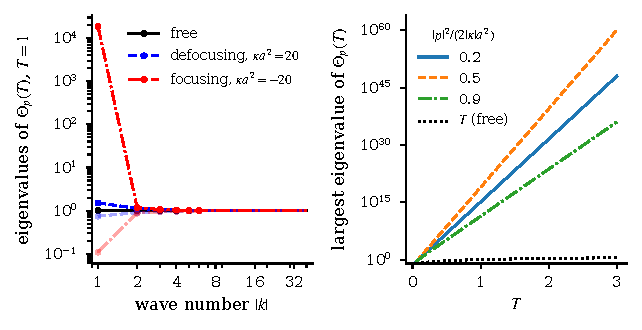
\includegraphics[width=\textwidth]{mf_nls}
\caption{Left: the two eigenvalues of the per pair information block $\Theta_p(T)$ of Proposition~\ref{m:prop:bog} at $T=1$ against the wave number $|k|$, where $|p|^2=4\pi^2|k|^2$; the larger eigenvalue is the dark curve and the smaller the pale curve of the same style. Free flow: both equal $T$. Defocusing case $\kappa a^2=20$: a compact perturbation decaying like $|p|^{-2}$, with eigenvalues $0.746$ and $1.511$ at $|k|=1$ and $0.998$ and $1.002$ at $|k|=16$. Focusing case $\kappa a^2=-20$: the mode $|k|=1$ lies inside the modulational band, $|p|^2=\lambda_1=4\pi^2<2|\kappa|a^2=40$, and its eigenvalues are $0.109$ and $1.87\times10^4$, so the larger one is amplified and the smaller one stays of order $1/(2\gamma_p)$. Right: growth in $T$ of the largest eigenvalue for $|p|^2/(2|\kappa|a^2)=0.2$, $0.5$, $0.9$ in the unstable band with $\kappa a^2=-0.6\lambda_1$ (on the unit torus only $|k|=1$ lies in this band, at the ratio $0.83$, so the three values illustrate the growth law rather than particular modes), against the free value $T$. Modulational instability amplifies the information about the initial condition exponentially along one direction, the opposite of the viscous curse of Table~\ref{m:tab:iota}.}\label{m:fig:nls}
\end{figure}

The consequences for the theory, illustrated in Figure~\ref{m:fig:nls}:
\begin{itemize}[nosep]
\item Defocusing. $\I^*_{\theta_0}\I_{\theta_0}=T\cdot\Id+\Kcal$ with $\Kcal$ block diagonal, $\norm{\Kcal_p}=O(\kappa a^2T/|p|^2)$, hence compact and two derivatives smoothing, which is the same order as in the parabolic case. Lemma~\ref{m:lem:bogmin} bounds the smallest eigenvalue of every block below, uniformly in $p$, so $\I^*_{\theta_0}\I_{\theta_0}$ is bounded above and below on $L^2$ and on every $H^\eta$, with explicit constants (Corollary~\ref{m:cor:condE}(a)). This is the analogue of Condition 2F without the factor $\Delta$, with $\eta_0=0$. The same bound is a stability estimate for the \emph{linearization} (Corollary~\ref{m:cor:condE}(b)). It is not Condition 2E, which is a lower bound on the increments of the nonlinear map $\Gcal$ and follows instead from an energy estimate for the difference of two solutions (Proposition~\ref{m:prop:nlsstab}); Remark~\ref{m:rem:condEgap} states precisely what is and is not verified. Granting the remaining conditions, the Bernstein von Mises limit is $\Ncal_{\theta_0}=N(0,T\diag\Theta_p(T)^{-1})$, whose per block covariance $T\Theta_p(T)^{-1}$ is bounded uniformly in $p$ \emph{and} in $T$ (Corollary~\ref{m:cor:condE}(c)); the limit is tight on $H^{-a}$ for $a>d/2$, and the trajectory theorem holds in weak topologies and for functionals but not in supremum norm, as in the linear case.
\item Focusing. For modes with $|p|^2<2|\kappa|a^2$ the largest eigenvalue of the block grows like $e^{2\gamma_pT}$ (Proposition~\ref{m:prop:bog}), so the component of the initial condition along the corresponding eigenvector is recovered with variance of order $Te^{-2\gamma_pT}/N$: the instability amplifies information, but along one direction of each unstable block only. The other direction is damped by the same flow, the smallest eigenvalue stays near $1/(2\gamma_p)$ (Lemma~\ref{m:lem:bogmin}(vi)), and the variance of that component is of order $2\gamma_pT/N$, which grows with $T$. There are finitely many such modes, so the tightness of the limit is not affected. The price is that the constants in Conditions 2A and 2D, which concern the nonlinear map, and the quadratic remainder of Condition 2C can be expected to grow with $T$, so that the localization set of Theorem~3 of Nickl~\cite{nicklbvm2024} would have to shrink accordingly; a Bernstein von Mises theorem can be expected only for $T$ fixed and $N\to\infty$, with constants exponential in $\gamma_{\max}T$. Computationally the curvature constant $c_{\min}$ of Nickl and Wang, the smallest eigenvalue of the normalized block $\Theta_p(T)/T$, does not become large: it is of order $1/(2\gamma_pT)$, and the amplification appears instead in the condition number $\lambda_{\max}/\lambda_{\min}$ of the block (Lemma~\ref{m:lem:bogmin}(vi)).
\item General backgrounds. For $u_0$ with several Fourier modes the conjugation term couples $p$ to $2k_0-p$ for every mode $k_0$ of $u_0$, and the time integrals in $\I^*\I$ are of the form $\int_0^Te^{i(\lambda_{p}+\lambda_{p'}-\lambda_{k_0}-\lambda_{k_0'})t}dt$: they are $O(1)$ on the four wave resonant manifold $\lambda_{k_1}+\lambda_{k_2}=\lambda_{k_3}+\lambda_{k_4}$, $k_1+k_2=k_3+k_4$, and $O(1/|\text{mismatch}|)$ off it. The resonant part is not compact in general; on $\T^2$ the resonant manifold is large. This is the structure that the wave turbulence derivation of Deng and Hani~\cite{denghani2023} exploits, and the invertibility of the information operator for a general NLS background is a question about the same resonant sums.
\item Sufficient statistic and GBC. Unchanged in form: the one step statistic \eqref{m:eq:onestep} with the adjoint of \eqref{m:eq:nlslin}, with $u_0=u_{\bar\theta_N}$. For the real inner product $\mathrm{Re}\int A\bar B$, multiplication by $i$ is skew and $U\mapsto c\bar U$ is self adjoint for every function $c$, so the adjoint of the generator $U\mapsto i\Delta U-i\kappa(2|u_0|^2U+u_0^2\bar U)$ of \eqref{m:eq:nlslin} is $W\mapsto-i\Delta W+i\kappa(2|u_0|^2W-u_0^2\bar W)$. Hence, for a source $g$ on $\mathcal X$, in \eqref{m:eq:onestep} the residuals $\sum_{i\in\mathcal I}r_i\,\delta_{X_i}$, the adjoint is $\I^*g=W(0)$, where $W$ solves the backward problem $i\partial_tW+\Delta W=\kappa(2|u_0|^2W-u_0^2\bar W)-ig$, $W(T)=0$: then $\frac{d}{dt}\mathrm{Re}\langle U,W\rangle=-\mathrm{Re}\langle U,g\rangle$ for the solution $U$ of \eqref{m:eq:nlslin}, so that $\int_0^T\mathrm{Re}\langle U(t),g(t)\rangle dt=\mathrm{Re}\langle h,W(0)\rangle$. If a Bernstein von Mises theorem holds (Remark~\ref{m:rem:condEgap}), the GBC quantile map is asymptotically affine with per pair scale $T\Theta_p(T)^{-1}/N$ about a plane wave, and a generator with $2\times2$ block structure over Fourier pairs is exact to leading order.
\end{itemize}

\subsubsection{The smallest eigenvalue of a Bogoliubov block} The blocks of Proposition~\ref{m:prop:bog} are $2\times2$, so their spectrum is determined by two scalars, and the determinant is fixed by a conservation law rather than by a computation: the Bogoliubov flow is area preserving, $\det M_p(t)=1$ for every $p$ and every $t$, in the elliptic, hyperbolic and degenerate cases alike. This is the linearized form of the conservation of the symplectic form $\mathrm{Im}\int U\bar W$ noted after \eqref{m:eq:nlslin}.

\begin{lemma}[Determinant, trace and smallest eigenvalue of $\Theta_p(T)$]\label{m:lem:bogmin}
Let $\Theta_p(T)=\int_0^TM_p(t)^\top M_p(t)\,dt$ be the block of Proposition~\ref{m:prop:bog}, and write $\omega=\omega_p$, $r=r_p=\omega_p/|p|^2$ in the elliptic case $\omega_p^2>0$, and $\gamma=\gamma_p=|\omega_p|$, $\rho=\rho_p=\gamma_p/|p|^2$ in the hyperbolic case $\omega_p^2<0$. Then, for every $T>0$:
\begin{enumerate}[label=(\roman*),nosep,leftmargin=2.2em]
\item $\det M_p(t)=1$ for all $t$, and consequently
\[
\det\Theta_p(T)\ \ge\ T^2\qquad\text{for every }p\text{ and every }T>0,
\]
with no restriction on $\omega_pT$.
\item Explicitly, for $p\ne0$ in the elliptic case,
\[
\det\Theta_p(T)=T^2+\frac{(r-r^{-1})^2}{4}\Big(T^2-\frac{\sin^2\omega T}{\omega^2}\Big),
\]
and in the hyperbolic case $\det\Theta_p(T)=T^2+\frac{(\rho+\rho^{-1})^2}{4}\big(\gamma^{-2}\sinh^2\gamma T-T^2\big)$, which is the analytic continuation $\omega\mapsto i\gamma$, $r\mapsto i\rho$ of the first formula. At $p=0$, $\Theta_0(T)=T\left(\begin{smallmatrix}1+\frac43s^2&-s\\-s&1\end{smallmatrix}\right)$ with $s=\kappa a^2T$, so $\det\Theta_0(T)=T^2(1+\tfrac13s^2)$.
\item In the elliptic case $\tr\,\Theta_p(T)=2T+(r-r^{-1})^2\int_0^T\sin^2\omega t\,dt\le T(r^2+r^{-2})$, and $\tr\,\Theta_0(T)=T(2+\tfrac43s^2)$.
\item Since $\Theta_p(T)$ is a positive definite $2\times2$ matrix, $\lambda_{\min}=\det/\lambda_{\max}\ge\det/\tr$, whence in the elliptic case
\[
\lambda_{\min}\big(\Theta_p(T)\big)\ \ge\ \frac{T}{r_p^2+r_p^{-2}},\qquad\text{and}\qquad \lambda_{\min}\big(\Theta_0(T)\big)\ \ge\ \frac T4 .
\]
If $r_p\ge1$ this implies $\lambda_{\min}\ge T/(1+r_p^2)$; if $r_p<1$ the form $T/(1+r_p^2)$ is false, so $r_p^2+r_p^{-2}$ cannot be replaced by $1+r_p^2$ in general.
\item Defocusing case, $\kappa>0$. Then $1<r_p^2\le1+2\kappa a^2/\lambda_1$ for $p\ne0$, with $\lambda_1=4\pi^2$ the smallest nonzero eigenvalue of $-\Delta$, and
\[
\begin{gathered}
\inf_p\lambda_{\min}\big(\Theta_p(T)\big)\ \ge\ \frac{T\lambda_1}{4(\lambda_1+\kappa a^2)},\\
\sup_{p\ne0}\lambda_{\max}\big(\Theta_p(T)\big)\ \le\ \frac{2T(\lambda_1+\kappa a^2)}{\lambda_1}.
\end{gathered}
\]
\item Focusing band, $\omega_p^2<0$. As $\gamma_pT\to\infty$, $\lambda_{\max}\big(\Theta_p(T)\big)\sim\tr\,\Theta_p(T)\sim(\rho_p+\rho_p^{-1})^2e^{2\gamma_pT}/(8\gamma_p)$ and $\lambda_{\min}\big(\Theta_p(T)\big)=\det\Theta_p(T)/\lambda_{\max}\to1/(2\gamma_p)$. The bound $\lambda_{\min}\ge T^2/\tr\,\Theta_p(T)$ still holds but is exponentially small in $\gamma_pT$, so it is far from sharp: the amplification is confined to one eigendirection, and the block is well conditioned in determinant and badly conditioned in ratio, with condition number $\lambda_{\max}/\lambda_{\min}\sim\frac14(\rho_p+\rho_p^{-1})^2e^{2\gamma_pT}$.
\end{enumerate}
\end{lemma}

\begin{proof}
(i) The generator $A_p$ in \eqref{m:eq:bog} has $\tr\,A_p=0$, so Liouville's formula gives $\det M_p(t)=e^{t\,\tr\,A_p}=1$. Hence $P(t):=M_p(t)^\top M_p(t)$ is symmetric positive definite with $\det P(t)=1$ for every $t$. Minkowski's determinant inequality, $\det(A+B)^{1/2}\ge(\det A)^{1/2}+(\det B)^{1/2}$ for positive semidefinite $2\times2$ matrices $A,B$, says that $P\mapsto(\det P)^{1/2}$ is superadditive on the cone; applying it to Riemann sums for $\int_0^TP(t)\,dt$ and passing to the limit,
\[
\big(\det\Theta_p(T)\big)^{1/2}\ \ge\ \int_0^T\big(\det P(t)\big)^{1/2}dt\ =\ T .
\]

(ii) to (iii) Write $C=\cos\omega t$, $S=\sin\omega t$ and
\[
\begin{gathered}
\alpha=\int_0^TC^2=\frac T2+\frac{\sin2\omega T}{4\omega},\qquad
\beta=\int_0^TS^2=\frac T2-\frac{\sin2\omega T}{4\omega},\\
\mu=\int_0^TSC=\frac{\sin^2\omega T}{2\omega},
\end{gathered}
\]
so that $\alpha+\beta=T$. By the entries of $M_p^\top M_p$ recorded in Proposition~\ref{m:prop:bog}, $\Theta_{11}=\alpha+r^2\beta$, $\Theta_{22}=\alpha+r^{-2}\beta$ and $\Theta_{12}=(r^{-1}-r)\mu$. Using $r^2+r^{-2}=2+(r-r^{-1})^2$,
\[
\begin{aligned}
\det\Theta_p&=(\alpha+r^2\beta)(\alpha+r^{-2}\beta)-(r-r^{-1})^2\mu^2\\
&=(\alpha+\beta)^2+(r-r^{-1})^2\big(\alpha\beta-\mu^2\big),
\end{aligned}
\]
and, with $\sin^22\omega T=4\sin^2\omega T\cos^2\omega T$,
\[
\begin{aligned}
\alpha\beta-\mu^2&=\frac{T^2}4-\frac{\sin^22\omega T}{16\omega^2}-\frac{\sin^4\omega T}{4\omega^2}\\
&=\frac{T^2}4-\frac{\sin^2\omega T}{4\omega^2}\big(\cos^2\omega T+\sin^2\omega T\big)
=\frac14\Big(T^2-\frac{\sin^2\omega T}{\omega^2}\Big),
\end{aligned}
\]
which is the stated determinant and, since $|\sin x|\le|x|$, recovers $\det\Theta_p\ge T^2$ with the deficit exhibited. Likewise $\tr\,\Theta_p=2\alpha+(r^2+r^{-2})\beta=2(\alpha+\beta)+(r-r^{-1})^2\beta=2T+(r-r^{-1})^2\beta$, and $\beta\le T$ gives $\tr\,\Theta_p\le T\big(2+(r-r^{-1})^2\big)=T(r^2+r^{-2})$. The hyperbolic case is the same computation with $C,S$ replaced by $\cosh\gamma t,\sinh\gamma t$. The diagonal weights of $M_p^\top M_p$ are then $\cosh^2+\rho^2\sinh^2$ and $\cosh^2+\rho^{-2}\sinh^2$, the off diagonal weight is $(\rho+\rho^{-1})\sinh\cosh$ in place of $(r^{-1}-r)\sin\cos$, and with
\[
\begin{gathered}
\alpha_h=\int_0^T\cosh^2\gamma t\,dt=\frac T2+\frac{\sinh2\gamma T}{4\gamma},\\
\beta_h=\int_0^T\sinh^2\gamma t\,dt=-\frac T2+\frac{\sinh2\gamma T}{4\gamma},\\
\mu_h=\int_0^T\sinh\gamma t\cosh\gamma t\,dt=\frac{\sinh^2\gamma T}{2\gamma}
\end{gathered}
\]
one has $\alpha_h-\beta_h=T$ in place of $\alpha+\beta=T$, $\det\Theta_p=(\alpha_h-\beta_h)^2+(\rho+\rho^{-1})^2(\alpha_h\beta_h-\mu_h^2)$, $\tr\,\Theta_p=2\alpha_h+(\rho^2+\rho^{-2})\beta_h$, and $\alpha_h\beta_h-\mu_h^2=\frac14(\gamma^{-2}\sinh^2\gamma T-T^2)\ge0$ because $\sinh x\ge x$. At $p=0$ the generator is nilpotent, $M_0(t)=\left(\begin{smallmatrix}1&0\\-2\kappa a^2t&1\end{smallmatrix}\right)$, and integrating $M_0^\top M_0$ gives the stated $\Theta_0(T)$.

(iv) For a positive definite $2\times2$ matrix, $\lambda_{\min}\lambda_{\max}=\det$ and $\lambda_{\max}\le\lambda_{\min}+\lambda_{\max}=\tr$, so $\lambda_{\min}=\det/\lambda_{\max}\ge\det/\tr$; combining (i) and (iii) gives $\lambda_{\min}\ge T^2/\big(T(r^2+r^{-2})\big)$. At $p=0$, $\det/\tr=T(3+s^2)/(6+4s^2)$, which decreases from $T/2$ at $s=0$ to $T/4$ as $s\to\infty$ and is therefore always at least $T/4$. For $r\ge1$ one has $r^{-2}\le1$, so $r^2+r^{-2}\le1+r^2$ and the weaker bound follows; for $r<1$ the inequality reverses and $T/(1+r^2)$ is not a valid bound: as $r\downarrow0$ with $|p|^2$ fixed, $M_p(t)\to\left(\begin{smallmatrix}1&|p|^2t\\0&1\end{smallmatrix}\right)$, for which $\det\Theta_p=T^2+|p|^4T^4/12$ and $\tr\,\Theta_p=2T+|p|^4T^3/3$, so $\lambda_{\min}\to T/4$ as $|p|^2T\to\infty$ while $T/(1+r^2)\to T$.

(v) In the defocusing case $r_p^2=1+2\kappa a^2/|p|^2>1$ is decreasing in $|p|$, hence $r_p^2\le R:=1+2\kappa a^2/\lambda_1$ for $p\ne0$; $x\mapsto x+x^{-1}$ is increasing on $[1,\infty)$, so $r_p^2+r_p^{-2}\le R+R^{-1}\le R+1=2(\lambda_1+\kappa a^2)/\lambda_1$, and (iv) gives $\lambda_{\min}\ge T\lambda_1/\big(2(\lambda_1+\kappa a^2)\big)$ for $p\ne0$. That exceeds $T\lambda_1/\big(4(\lambda_1+\kappa a^2)\big)$, and so does the bound $T/4$ at $p=0$ because $\lambda_1<\lambda_1+\kappa a^2$; taking the minimum over the two cases gives the first display. The second is $\lambda_{\max}\le\tr\,\Theta_p\le T(r_p^2+r_p^{-2})$ with the same estimate.

(vi) By (ii) and $\sinh^2x\sim e^{2x}/4$, $\det\Theta_p(T)\sim(\rho+\rho^{-1})^2e^{2\gamma T}/(16\gamma^2)$, and since $\alpha_h,\beta_h\sim e^{2\gamma T}/(8\gamma)$, $\tr\,\Theta_p(T)=2\alpha_h+(\rho^2+\rho^{-2})\beta_h\sim(2+\rho^2+\rho^{-2})e^{2\gamma T}/(8\gamma)=(\rho+\rho^{-1})^2e^{2\gamma T}/(8\gamma)$. Hence $\det/\tr\to1/(2\gamma)$ and $\det/\tr^2\to0$, and from $\lambda_{\min}=2\det/\big(\tr+\sqrt{\tr^2-4\det}\big)$ we get $\lambda_{\min}=(\det/\tr)(1+o(1))\to1/(2\gamma)$ and $\lambda_{\max}=\tr\,(1+o(1))$. The condition number is $\lambda_{\max}/\lambda_{\min}=\lambda_{\max}^2/\det\sim\frac14(\rho+\rho^{-1})^2e^{2\gamma T}$.
\end{proof}

If observation starts at $T_0>0$, the information on $[T_0,T]$ is $\int_{T_0}^TM_p^\top M_p\,dt$, and Lemma~\ref{m:lem:bogmin} says what survives. For a stable mode with $p\ne0$ the proofs of (i), (iii) and (iv) use only $\det M_p(t)=1$ and the pointwise bound $\tr\big(M_p(t)^\top M_p(t)\big)\le r_p^2+r_p^{-2}$, so the bounds hold with $T$ replaced by $T-T_0$: the position of the window does not enter them, as in the linear case. Two things change. In the focusing band the damped eigenvector $v$ of $A_p$ satisfies $M_p(t)v=e^{-\gamma_pt}v$, so the Rayleigh quotient gives $\lambda_{\min}\big(\int_{T_0}^TM_p^\top M_p\,dt\big)\le e^{-2\gamma_pT_0}/(2\gamma_p)$: a late window loses the information along the damped direction, as in the dissipation barrier of Table~\ref{m:tab:iota}, but for the finitely many unstable modes only (for $\kappa a^2=-20$, $|k|=1$ and windows of length one the bound is sharp to within one percent). At $p=0$ the shear $M_0(t)$ grows linearly: with $\tau=T-T_0$ the window block has determinant $\tau^2\big(1+\tfrac13\kappa^2a^4\tau^2\big)$ and trace $\tau\big(2+\tfrac43\kappa^2a^4(T^2+TT_0+T_0^2)\big)$, so its smallest eigenvalue decays like $T_0^{-2}$, for the single mode $p=0$.

\begin{corollary}[Linearized stability and the analogue of Condition 2F for the defocusing plane wave]\label{m:cor:condE}
Let $\kappa>0$, $\theta_0=a$ constant, and let $\I_{\theta_0}$ be the linearization \eqref{m:eq:nlslin}, with adjoint taken with respect to unnormalized $L^2(\mathcal X)$, $\mathcal X=[0,T]\times\T^d$. Set
\[
c_\star^2=\frac{T\lambda_1}{4(\lambda_1+\kappa a^2)},\qquad
C_\star^2=\max\Big\{\frac{2T(\lambda_1+\kappa a^2)}{\lambda_1},\ T\big(2+\tfrac43\kappa^2a^4T^2\big)\Big\}.
\]
Then for every $h\in L^2(\T^d;\C)$,
\[
c_\star^2\norm{h}_{L^2(\Omega)}^2\ \le\ \norm{\I_{\theta_0}h}^2_{L^2(\mathcal X)}=\big\langle h,\I^*_{\theta_0}\I_{\theta_0}h\big\rangle\ \le\ C_\star^2\norm{h}_{L^2(\Omega)}^2,
\]
and consequently
\begin{enumerate}[label=(\alph*),nosep,leftmargin=2.2em]
\item $\I^*_{\theta_0}\I_{\theta_0}$ is a homeomorphism of $H^\eta(\T^d)$ for every $\eta\in\R$, with the explicit constants $c_\star^2,C_\star^2$; this is the analogue of Condition 2F without the factor $\Delta$, with $\eta_0=0$, and no smoothing is needed, while Condition 2F as stated fails, since $\Delta\I^*_{\theta_0}\I_{\theta_0}$ loses two derivatives;
\item the linearization satisfies the stability estimate
\[
\norm{\I_{\theta_0}h}_{L^2(\mathcal X)}\ \ge\ c_\star\norm{h}_{L^2(\Omega)}\ \ge\ c_\star\norm{h}_{H^{-1}(\Omega)} ,
\]
which is the estimate of Condition 2E with $\I_{\theta_0}$ in place of $\Gcal$, in the stronger norm $L^2$ rather than $H^{-1}$;
\item $\Ncal_{\theta_0}=N\big(0,T(\I^*_{\theta_0}\I_{\theta_0})^{-1}\big)=N\big(0,T\diag\Theta_p(T)^{-1}\big)$ has per block covariance $T\Theta_p(T)^{-1}$ with
\[
\norm{T\Theta_p(T)^{-1}}\ \le\ \frac{T}{\lambda_{\min}(\Theta_p(T))}\ \le\ \frac{4(\lambda_1+\kappa a^2)}{\lambda_1}
\]
uniformly in $p$ and in $T$, so $\Ncal_{\theta_0}$ is tight on $H^{-a}$ for $a>d/2$; contrast the parabolic case, where $1/\iota_j\asymp2\nu\lambda_jT$ diverges with $j$ and with $T$.
\end{enumerate}
\end{corollary}

\begin{proof}
The Bogoliubov substitution $U=e^{-i\kappa a^2t}(\phi+i\psi)$ is at each $t$ a pointwise rotation of $\C\cong\R^2$, hence an isometry of $L^2(\T^d;\C)$, and $\norm{h}^2_{L^2(\Omega)}=\norm{\phi(0)}^2+\norm{\psi(0)}^2$ for $h=U(0)$, the norms being those of the real functions $\phi(0),\psi(0)$. Because the design is uniform on $\mathcal X$, whose measure is $T$, and the adjoint is unnormalized,
\[
\begin{aligned}
\norm{\I_{\theta_0}h}^2_{L^2(\mathcal X)}&=\int_0^T\norm{U(t)}^2_{L^2(\T^d)}dt=\sum_p\int_0^T\big|M_p(t)v_p\big|^2dt\\
&=\sum_p\big\langle v_p,\Theta_p(T)v_p\big\rangle,\qquad v_p=\big(\phi_p(0),\psi_p(0)\big),
\end{aligned}
\]
with $\sum_p|v_p|^2=\norm{h}^2_{L^2(\Omega)}$ by Parseval. The two sided bound is Lemma~\ref{m:lem:bogmin}(v) applied term by term, together with $\lambda_{\max}(\Theta_0(T))\le\tr\,\Theta_0(T)=T(2+\frac43\kappa^2a^4T^2)$ for the zero mode. For (a), each block acts within a single $p$ and therefore commutes with the Sobolev weights $(1+\lambda_p)^{\eta/2}$, so the two sided bound on $L^2$ transfers to $H^\eta$ for every $\eta$. Part (b) is the left inequality together with $\norm{h}_{H^{-1}}\le\norm{h}_{L^2}$. Part (c) is the block inverse, with tightness as in Proposition~\ref{m:prop:sch}: $\sum_p\lambda_p^{-a}<\infty$ for $a>d/2$.
\end{proof}

The stability estimate for $\Gcal$ itself does not go through the linearization.

\begin{proposition}[Stability of the cubic NLS solution map]\label{m:prop:nlsstab}
Let $\kappa\ne0$, let $u$ and $v$ solve $i\partial_tu+\Delta u=\kappa|u|^2u$ on $[0,T]\times\T^d$ with data $\theta$ and $\vartheta$, in $H^1$ if $d=1$ and in $H^2$ if $d=2$, and suppose that $\norm{u(t)}_{L^\infty}\le M_\infty$ and $\norm{v(t)}_{L^\infty}\le M_\infty$ for $t\le T$, with $M_\infty>0$. Then, for $t\le T$,
\[
e^{-6|\kappa|M_\infty^2t}\norm{\theta-\vartheta}^2_{L^2(\Omega)}\ \le\ \norm{u(t)-v(t)}^2_{L^2(\Omega)}\ \le\ e^{6|\kappa|M_\infty^2t}\norm{\theta-\vartheta}^2_{L^2(\Omega)},
\]
and, with the unnormalized $L^2(\mathcal X)$ of Corollary~\ref{m:cor:condE},
\[
\begin{aligned}
\norm{\Gcal(\theta)-\Gcal(\vartheta)}^2_{L^2(\mathcal X)}&\ge\frac{1-e^{-6|\kappa|M_\infty^2T}}{6|\kappa|M_\infty^2}\norm{\theta-\vartheta}^2_{L^2(\Omega)}\\
&\ge Te^{-6|\kappa|M_\infty^2T}\norm{\theta-\vartheta}^2_{H^{-1}(\Omega)} .
\end{aligned}
\]
A bound $M_\infty=M_\infty(T,\kappa,B)$ that holds for all data in a ball of radius $B$ exists in each of the following cases:
\begin{enumerate}[label=(\alph*),nosep,leftmargin=2.2em]
\item $d=1$, either sign of $\kappa$, every ball of $H^1$;
\item $d=2$, $\kappa>0$, every ball of $H^2$;
\item $d=2$, $\kappa<0$, the balls of $H^2$ with $2|\kappa|C_2B^2T<1$, where $C_2$ is a constant such that $\norm{|f|^2f}_{H^2}\le C_2\norm f^3_{H^2}$.
\end{enumerate}
On such a ball, Condition 2E therefore holds for $\Gcal$, with the stronger norm $L^2$ on the right and the constant $T^{1/2}e^{-3|\kappa|M_\infty^2T}$, Condition 2A holds with the bound $M_\infty$, and the upper bound gives the $L^2$ Lipschitz estimate of Condition 2B, $\norm{\Gcal(\theta)-\Gcal(\vartheta)}^2_{L^2(\mathcal X)}\le\big(e^{6|\kappa|M_\infty^2T}-1\big)\norm{\theta-\vartheta}^2_{L^2(\Omega)}/(6|\kappa|M_\infty^2)$.
\end{proposition}

\begin{proof}
Write $f(z)=|z|^2z$ and $w=u-v$. Since $|\partial_zf|+|\partial_{\bar z}f|=3|z|^2$, pointwise
\[
|f(u)-f(v)|\ \le\ 3|w|\int_0^1|v+sw|^2ds\ \le\ \tfrac32\big(|u|^2+|v|^2\big)|w| .
\]
The difference solves $\partial_tw=i\Delta w-i\kappa\big(f(u)-f(v)\big)$, and $i\Delta$ is skew for the real inner product $\mathrm{Re}\langle\cdot,\cdot\rangle$ of $L^2(\Omega)$, so
\[
\Big|\frac d{dt}\norm{w}^2_{L^2(\Omega)}\Big|=2|\kappa|\,\big|\mathrm{Re}\big\langle f(u)-f(v),iw\big\rangle\big|\le6|\kappa|M_\infty^2\norm{w}^2_{L^2(\Omega)},
\]
and Gr\"onwall's inequality, forward and backward in time, gives the two sided bound. For the uniform design $\norm{\Gcal(\theta)-\Gcal(\vartheta)}^2_{L^2(\mathcal X)}=\int_0^T\norm{w(t)}^2_{L^2(\Omega)}dt$, so integrating the lower bound gives the first inequality of the second display, $(1-e^{-x})/x\ge e^{-x}$ and $\norm\cdot_{H^{-1}}\le\norm\cdot_{L^2}$ give the second, and integrating the upper bound gives the Lipschitz estimate.

(a) The mass $m=\norm{u(t)}^2_{L^2}$ and the energy $E=\norm{\partial_xu(t)}^2_{L^2}+\frac\kappa2\norm{u(t)}^4_{L^4}$ do not depend on $t$, and on the circle of length one $\norm g^2_{L^\infty}\le\norm g^2_{L^2}+2\norm g_{L^2}\norm{\partial_xg}_{L^2}$, so that $m$ and $E$ are bounded on the ball. If $\kappa>0$, then $\norm{\partial_xu(t)}^2_{L^2}\le E$. If $\kappa<0$, the same inequality gives $\norm{u}^4_{L^4}\le\norm u^2_{L^\infty}\norm u^2_{L^2}\le m^2+2m^{3/2}\norm{\partial_xu}_{L^2}$, so $y=\norm{\partial_xu(t)}_{L^2}$ satisfies $y^2\le E+|\kappa|(m^2/2+m^{3/2}y)$, a quadratic inequality that bounds $y$. In both cases $\norm{u(t)}_{H^1}$ is bounded for all $t$ by a function of $B$ and $\kappa$, which also continues the local solution to all times, and the inequality above bounds $\norm{u(t)}_{L^\infty}$. (b) Since $\sqrt\kappa\,u$ solves $i\partial_tu+\Delta u=|u|^2u$, Theorem~1.1 of Planchon, Tzvetkov and Visciglia~\cite{ptv2017}, applied to the $H^2$ norm, bounds $\sup_{t\le T}\norm{u(t)}_{H^2}$ in terms of $T$ and $\norm\theta_{H^2}$ (their argument also gives the global existence that the theorem assumes), and $H^2(\T^2)\subset L^\infty$. (c) Since $i\Delta$ commutes with $1-\Delta$, it is skew in $H^2$ as well, and $y(t)=\norm{u(t)}^2_{H^2}$ satisfies $y'\le2|\kappa|\norm{f(u)}_{H^2}\norm u_{H^2}\le2|\kappa|C_2y^2$; hence $y(t)\le y(0)/(1-2|\kappa|C_2y(0)t)\le B^2/(1-2|\kappa|C_2B^2T)$ on $[0,T]$, which also continues the local solution to $[0,T]$, and again $H^2(\T^2)\subset L^\infty$.
\end{proof}

\begin{remark}[What is verified, what is not, and what would close the gap]\label{m:rem:condEgap}
Condition 2E, as recorded in Section~\ref{m:sec:papers}, is the estimate $\norm{\Gcal(\theta)-\Gcal(\theta_0)}_{L^2(\mathcal X)}\ge c\norm{\theta-\theta_0}_{H^{-1}}$ for the \emph{nonlinear} solution map $\Gcal$, required uniformly over the Sobolev ball supporting the prior. Corollary~\ref{m:cor:condE}(b) is that estimate for $\I_{\theta_0}=D\Gcal_{\theta_0}$, the derivative at a single point. The two statements are different and neither implies the other; the second is a local injectivity and curvature statement about the tangent space of the solution manifold at $u_{\theta_0}$, not an identifiability statement about $\Gcal$.

Three things separate them. First, the passage from the derivative to the secant is only local. Along the segment $\vartheta_s=\theta_0+s(\theta-\theta_0)$,
\[
\begin{aligned}
\Gcal(\theta)-\Gcal(\theta_0)&=\int_0^1\I_{\vartheta_s}(\theta-\theta_0)\,ds\\
&=\I_{\theta_0}(\theta-\theta_0)+\int_0^1\big(\I_{\vartheta_s}-\I_{\theta_0}\big)(\theta-\theta_0)\,ds ,
\end{aligned}
\]
so if the linearization were Lipschitz in its base point, $\norm{(\I_\vartheta-\I_{\theta_0})h}_{L^2(\mathcal X)}\le L\norm{\vartheta-\theta_0}_{H^\zeta}\norm{h}_{L^2}$ for some $\zeta>d/2$ and all $\vartheta$ on the segment, then Corollary~\ref{m:cor:condE}(b) would give
\[
\norm{\Gcal(\theta)-\Gcal(\theta_0)}_{L^2(\mathcal X)}\ \ge\ \Big(c_\star-\tfrac L2\norm{\theta-\theta_0}_{H^\zeta}\Big)\norm{\theta-\theta_0}_{L^2(\Omega)} ,
\]
that is, Condition 2E with constant $c_\star/2$ and with the stronger norm $L^2$ on the right, but only on $\{\norm{\theta-\theta_0}_{H^\zeta}\le c_\star/L\}$. Nothing above bounds $L$ for cubic NLS; $L$ depends on $T$ and on $\norm{\theta}_{H^\zeta}$, and in the focusing band the linearized flow itself varies on the scale $e^{\gamma_{\max}T}$, so such a radius can be expected to shrink exponentially in $T$.

Second, a local estimate is not Condition 2E. Condition 2E is global on the ball, and it is what excludes a second $\theta$ far from $\theta_0$ with $\Gcal(\theta)$ close to $\Gcal(\theta_0)$. For cubic NLS the global statement does not need the linearization: it is Proposition~\ref{m:prop:nlsstab}, on every ball on which the solutions stay bounded, which for $d\le2$ and $\kappa>0$ is every ball of $H^2$. The reason is the reverse of the parabolic one. The flow is unitary on $L^2$ and the nonlinearity is Lipschitz on bounded sets, so two solutions approach each other at most exponentially fast and the distance between their initial data is never lost, only reduced by the factor $e^{-3|\kappa|M_\infty^2t}$. For the heat equation and Navier Stokes the semigroup damps differences, which is why the right side of Condition 2E carries the weaker norm $H^{-1}$ there, by \eqref{m:eq:modeinfo} and by Konen and Nickl~\cite{konennickl2026} respectively.

Third, even the derivative estimate is proved only at the plane wave background. For a general $\theta_0$, $\I^*_{\theta_0}\I_{\theta_0}$ is no longer block diagonal, and its invertibility is the four wave resonant sum question of the third bullet above and of Open Question~\ref{m:op:planewave} below. The segment $\vartheta_s$ passes through such backgrounds even when both endpoints are plane waves, as soon as their wave vectors differ, so the first point above cannot be run at the plane wave alone.

The accounting for cubic NLS about a plane wave in the defocusing case is therefore: the analogue of Condition 2F without the factor $\Delta$ is verified with $\eta_0=0$ and explicit constants (Corollary~\ref{m:cor:condE}(a)), and Condition 2F itself fails, as for the linear equation; the linearized stability estimate is verified in $L^2$, hence a fortiori in $H^{-1}$ (Corollary~\ref{m:cor:condE}(b)); Condition 2E for $\Gcal$ is verified in $L^2$ on every ball of $H^2$, for $d\le2$, together with Condition 2A and the $L^2$ Lipschitz estimate of Condition 2B (Proposition~\ref{m:prop:nlsstab}); Conditions 2C and 2D are \emph{not} verified. Closing the gap requires the estimates of Conditions 2C and 2D, in particular a bound on the Lipschitz modulus of $\theta\mapsto\I_\theta$ from $H^\zeta$ into $\mathcal B\big(L^2(\Omega),L^2(\mathcal X)\big)$ on the localization set, which is a well posedness estimate for \eqref{m:eq:nlslin} with variable background, and a version of Theorem~\ref{m:thm:nickl2} under the analogue of Condition 2F without the factor $\Delta$.
\end{remark}


\subsection{The examples side by side}

Tables~\ref{m:tab:compare} and~\ref{m:tab:guarantee} collect the objects of Sections~\ref{m:sec:suff} to~\ref{m:sec:nondiss} for the heat equation, two dimensional Navier Stokes about the Taylor Green vortex, and the linear and cubic Schr\"odinger equations. The two dissipative columns differ only by a compact perturbation; the two dispersive columns differ from them in every row that involves smoothing or forgetting.

\begin{table}[tp]\centering\scriptsize
\setlength{\tabcolsep}{2pt}
\caption{Objects of the theory for the four examples, part one: the forward map, the information operator and the summary. $\lambda_j=4\pi^2|k_j|^2$; $\Theta_p(T)$ the Bogoliubov information block of Proposition~\ref{m:prop:bog}; $\Kcal$ compact. The $\I^*\I$ row is unnormalized ($\int_0^T$, as in \eqref{m:eq:modeinfo}) while $\iota_j$ is normalized ($\tfrac1T\int_0^T$, as in \eqref{m:eq:iota}). For cubic NLS the per mode information is the pair of eigenvalues of $T^{-1}\Theta_p(T)$, and the quantile map of the last row is conditional on a Bernstein von Mises theorem, which is not proved here (Remark~\ref{m:rem:condEgap}).}\label{m:tab:compare}
\begin{tabular}{>{\raggedright\arraybackslash}p{0.155\textwidth}>{\raggedright\arraybackslash}p{0.175\textwidth}>{\raggedright\arraybackslash}p{0.21\textwidth}>{\raggedright\arraybackslash}p{0.15\textwidth}>{\raggedright\arraybackslash}p{0.235\textwidth}}
\toprule
& Heat & Two dimensional Navier Stokes (Taylor Green) & Linear Schr\"odinger & Cubic NLS (plane wave)\\
\midrule
Forward map & $e^{\nu t\Delta}$ & nonlinear; $u_{\rm TG}$ exact & $e^{it\Delta}$, unitary & nonlinear, preserves the $L^2$ norm\\
Linearization $\I_{\theta_0}$ & $e^{\nu t\Delta}$ & Stokes $+$ nearest neighbor coupling $A|k|e^{-2\nu t}$ & $e^{it\Delta}$ itself & Bogoliubov $2\times2$ blocks \eqref{m:eq:bog}\\
$\I^*\I$ & $\diag(T\iota_j)$ & $\Lcal^*\Lcal+\Kcal$, $\Delta\Lcal^*\Lcal=(S_{2T}-\Id)/(2\nu)$ & $T\cdot\Id$ exactly & $\diag(\Theta_p(T))$, Prop.~\ref{m:prop:bog}\\
Per mode information & $\iota_j\asymp(2\nu\lambda_jT)^{-1}$ & same $+O\big(A/(\nu|k|)\big)$ & $1$ & defocusing: $1+O(\kappa a^2/|p|^2)$; focusing band: largest eigenvalue grows like $e^{2\gamma_pT}$, smallest is $\sim1/(2\gamma_pT)$\\
Effect of $T_0>0$ & factor $e^{-2\nu\lambda_jT_0}$ & same & none & no decay for stable modes with $p\ne0$; focusing band: damped direction at most $e^{-2\gamma_pT_0}/(2\gamma_p)$; $p=0$: smallest eigenvalue decays like $T_0^{-2}$, after Lem.~\ref{m:lem:bogmin}\\
Sufficient statistic & adjoint heat flow of data, exact & one step efficient score via adjoint linearized Navier Stokes & adjoint unitary flow of data, exact & one step efficient score via $W(0)$, with $W$ the backward solution of the adjoint of \eqref{m:eq:nlslin}\\
GBC quantile map & affine, scale $(N\iota_j+\rho^{-2}\lambda_j^\alpha)^{-1/2}$ for the limit Gram matrix $N\diag(\iota_j)$ & asymptotically affine, scale $T(\I^*\I)^{-1}/N$ & affine, scale $(N+\rho^{-2}\lambda_j^\alpha)^{-1/2}$ for the limit Gram matrix $N\,\Id$ & asymptotically affine, $2\times2$ block scale $T\Theta_p(T)^{-1}/N$\\
\bottomrule
\end{tabular}
\end{table}

\begin{table}[tp]\centering\scriptsize
\setlength{\tabcolsep}{2pt}
\caption{Objects of the theory for the four examples, part two: the limit theorems and the conditions. BvM stands for Bernstein von Mises. As in Table~\ref{m:tab:compare}, $\I^*\I$ is unnormalized and $\iota_j$ normalized, so that $\Ncal_{\theta_0}=N(0,T(\I^*\I)^{-1})=N(0,\diag(1/\iota_j))$ in every column; for cubic NLS $c_{\min}$ is the smallest eigenvalue of $T^{-1}\Theta_p(T)$ over the modes retained. The row on $c_{\min}$ gives the value of the curvature constant of the localized Langevin algorithm of Nickl and Wang~\cite{nicklwang2024} if their remaining conditions carry over (Section~\ref{sec:gradstab}). $^\dagger$For cubic NLS no Bernstein von Mises theorem is proved here: Conditions 2C and 2D are not verified, and Condition 2F holds only without the factor $\Delta$ (Remark~\ref{m:rem:condEgap}); Section~\ref{m:sec:nondiss} notes that the theorem can be expected for $T$ fixed.}\label{m:tab:guarantee}
\begin{tabular}{>{\raggedright\arraybackslash}p{0.155\textwidth}>{\raggedright\arraybackslash}p{0.175\textwidth}>{\raggedright\arraybackslash}p{0.21\textwidth}>{\raggedright\arraybackslash}p{0.15\textwidth}>{\raggedright\arraybackslash}p{0.235\textwidth}}
\toprule
& Heat & Two dimensional Navier Stokes (Taylor Green) & Linear Schr\"odinger & Cubic NLS (plane wave)\\
\midrule
BvM limit $\Ncal_{\theta_0}$ & $N(0,\diag(1/\iota_j))$ & $N(0,T(\I^*\I)^{-1})$ & $N(0,\Id)$ & $N(0,T\diag\Theta_p(T)^{-1})$\\
Tight on & $H^{-a}$, $a>1+d/2$ & $\Hds{-\beta}$, $\beta>2$ & $H^{-a}$, $a>d/2$ & $H^{-a}$, $a>d/2$\\
Trajectory BvM in sup norm & yes, $t>0$ & yes, $t>0$ & no & no\\
Trajectory BvM, weak topology & yes & yes & yes, Cor.~\ref{m:cor:schtransfer}(ii) & conjectural$^\dagger$\\
Functionals efficient at rate $\sqrt N$ & yes & yes & yes, Cor.~\ref{m:cor:schtransfer}(iv) & conjectural$^\dagger$ ($T$ fixed)\\
Nickl Wang $c_{\min}$, if the remaining conditions hold & $\min_j\iota_j\asymp D^{-2/d}$ & same & $1$ & defocusing: at least $\frac{\lambda_1}{4(\lambda_1+\kappa a^2)}$, uniformly in $D$ and $T$; focusing band: $\sim1/(2\gamma_pT)$\\
Condition 2E verified & yes, $\Gcal$ linear, \eqref{m:eq:modeinfo} gives it in $H^{-1}$ & Konen Nickl & yes, $\Gcal$ linear, in $L^2$ & yes, in $L^2$, on balls where the solutions stay bounded, which for $\kappa>0$ is every $H^2$ ball, Prop.~\ref{m:prop:nlsstab}; linearized form, Cor.~\ref{m:cor:condE}(b)\\
Condition 2F verified & trivially & Konen Nickl & fails; holds without the factor $\Delta$, as $\I^*\I=T\cdot\Id$ & fails; without the factor $\Delta$: plane wave, defocusing, Lem.~\ref{m:lem:bogmin}, Cor.~\ref{m:cor:condE}(a); general: open (resonances)\\
\bottomrule
\end{tabular}
\end{table}

\begin{proposition}[Linear Schr\"odinger transfer]\label{m:prop:sch}
For the linear Schr\"odinger equation, let the noise have independent standard Gaussian real and imaginary parts, let the prior be \eqref{m:eq:prior} truncated to the first $D=D_N$ modes, so that the real and the imaginary part of $\theta_j$ are independent with precision $\rho^{-2}\lambda_j^\alpha$, where $\rho^{-2}=N\delta_N^2$, $\alpha=\gamma$ and $\gamma>d/2$, let $\tilde\theta_N$ be the posterior mean, and write $N(0,\Id)$ for complex white noise whose real and imaginary parts are independent with covariance $\Id$. Then:
\begin{enumerate}[label=(\alph*),nosep,leftmargin=2.2em]
\item the posterior is exactly Gaussian, the adjoint summary $\Phi^*Y$ together with the design is exactly sufficient, and the GBC quantile map is exactly affine, with per mode scale $(N+\rho^{-2}\lambda_j^\alpha)^{-1/2}$ in the real and in the imaginary part when the Gram matrix $\Phi^*\Phi$ of the design is replaced by its limit $N\,\Id$;
\item if $D_N\to\infty$ and $D_N=o(N^{d/(2\gamma+d)})$, then $\Wone_{1,H^{-a}}\big(\Law(\sqrt N(\theta-\tilde\theta_N)\mid Z^{(N)}),N(0,\Id)\big)\to^P0$ for every $a>d/2$;
\item if in addition $\theta_0\in H^\gamma$ and $N\lambda_{D_N}^{-(a+\gamma)}\to0$, then $\sqrt N(\tilde\theta_N-\theta_0)\to^dN(0,\Id)$ in $H^{-a}$; the choice $D_N\asymp N^{d/(2\gamma+d)}/\log N$ meets the conditions of (b) and (c) for every $a>d/2$;
\item (b) and (c) hold with $u_\theta(t)$, $u_{\tilde\theta_N}(t)$ and $u_{\theta_0}(t)$ in place of $\theta$, $\tilde\theta_N$ and $\theta_0$, at every $t$ and uniformly in $t$, with the same limit $e^{it\Delta}_\#N(0,\Id)=N(0,\Id)$, and no supremum norm statement holds at any $t$.
\end{enumerate}
\end{proposition}

\begin{proof}
Write $\phi_i=\big(e^{i\lambda_jt_i}\overline{e_j(x_i)}\big)_{j\le D}$, so that $\Phi^*\Phi=\sum_i\phi_i\phi_i^*$ and $\Phi^*Y=\sum_i\phi_iY_i$, let $V_N=(\Phi^*\Phi+\rho^{-2}\Lambda^\alpha)^{-1}$, and let $P_D$ be the projection on the first $D$ modes.

(a) Up to a constant the log posterior density is $-\frac12(\theta-V_N\Phi^*Y)^*V_N^{-1}(\theta-V_N\Phi^*Y)$, so, as in Proposition~\ref{m:prop:linsuff}, the posterior is Gaussian with mean $\tilde\theta_N=V_N\Phi^*Y$, it depends on the data only through $\Phi^*Y$ and the design, and the real and imaginary parts of $\theta$ have the joint covariance $\left(\begin{smallmatrix}\mathrm{Re}V_N&-\mathrm{Im}V_N\\\mathrm{Im}V_N&\mathrm{Re}V_N\end{smallmatrix}\right)$. The real and the imaginary part of $\theta_j$ therefore have posterior variance $(V_N)_{jj}$, which is $(N+\rho^{-2}\lambda_j^\alpha)^{-1}$ when $\Phi^*\Phi=N\,\Id$, and the quantile map is that of \eqref{m:eq:linquant}.

(b) The $\phi_i$ are independent, their entries have modulus one, and $E[\phi_i\phi_i^*]=\Id$ because the $e_j$ are orthonormal and $x_i$ is uniform. The matrices $S_i=N^{-1}(\phi_i\phi_i^*-\Id)$ are centered, with $\norm{S_i}\le D/N$ and $\sum_iE[S_i^2]=N^{-1}(D-1)\Id$, so the matrix Bernstein inequality, Theorem~6.1.1 of Tropp~\cite{tropp2015}, gives for $\Gamma=N^{-1}\Phi^*\Phi-\Id$
\[
E\norm\Gamma\le\sqrt{\frac{2D\log(2D)}N}+\frac{D\log(2D)}{3N},
\]
which tends to zero because $D\log D=o(N)$. With $\Lambda_\delta=\delta_N^2\Lambda^\gamma=N^{-1}\rho^{-2}\Lambda^\alpha$ on the first $D$ modes, $NV_N=(\Id+\Lambda_\delta+\Gamma)^{-1}$ and $\Id+\Lambda_\delta\succeq\Id$, so on $\{\norm\Gamma<1\}$
\[
\norm{NV_N}\le\frac1{1-\norm\Gamma},\qquad\norm{NV_N-\Id}\le\frac{\norm\Gamma+\norm{\Lambda_\delta}}{1-\norm\Gamma},
\]
and $\norm{\Lambda_\delta}=\delta_N^2\lambda_D^\gamma\to0$ exactly when $D=o(N^{d/(2\gamma+d)})$, since $\lambda_D\asymp D^{2/d}$. Let $G$ have law $N(0,\Id)$. Then $(NV_N)^{1/2}P_DG$ has the posterior law of $\sqrt N(\theta-\tilde\theta_N)$, and for a matrix $A$ acting on the first $D$ modes $E\norm{AG}^2_{H^{-a}}=2\sum_j\lambda_j^{-a}(AA^*)_{jj}\le2\norm A^2\sum_{j\le D}\lambda_j^{-a}$. With $|\sqrt\mu-1|\le|\mu-1|$ for $\mu\ge0$, the square of the distance in (b) is therefore at most
\[
E\norm{(NV_N)^{1/2}P_DG-G}^2_{H^{-a}}\le2\norm{NV_N-\Id}^2\sum_j\lambda_j^{-a}+2\sum_{j>D}\lambda_j^{-a},
\]
which tends to zero in probability, because $\sum_j\lambda_j^{-a}<\infty$ for $a>d/2$.

(c) Write $Y=\Phi P_D\theta_0+r+\varepsilon$, where $r_i=u_{\theta_0-P_D\theta_0}(t_i,x_i)$ is the signal of the modes above $D$. Since $V_N\Phi^*\Phi=\Id-(NV_N)\Lambda_\delta$,
\[
\begin{aligned}
\sqrt N(\tilde\theta_N-\theta_0)&=\sqrt NV_N\Phi^*\varepsilon-\sqrt N(NV_N)\Lambda_\delta P_D\theta_0\\
&\quad+\sqrt NV_N\Phi^*r-\sqrt N(\theta_0-P_D\theta_0),
\end{aligned}
\]
and we take the four terms in turn; the norm of $H^{-a}$ is at most $\lambda_1^{-a/2}$ times that of $L^2$. Given the design, the first term is centered Gaussian, with the covariance structure of (a) for the matrix $(NV_N)(\Id+\Gamma)(NV_N)$, which tends to $\Id$ in operator norm, so the coupling of (b) shows that its law tends to $N(0,\Id)$ in $\Wone_{1,H^{-a}}$. In the second, $(NV_N)\Lambda_\delta=(\Id+\Lambda_\delta)^{-1}\Lambda_\delta-(NV_N)\Gamma(\Id+\Lambda_\delta)^{-1}\Lambda_\delta$. For the diagonal part, $b/(1+b)\le\min(1,b)\le b^{(a+\gamma)/(2\gamma)}$ for $b\ge0$ and $d/2<a\le\gamma$, so
\[
\begin{aligned}
N\norm{(\Id+\Lambda_\delta)^{-1}\Lambda_\delta P_D\theta_0}^2_{H^{-a}}&\le N\sum_j\lambda_j^{-a}\big(\delta_N^2\lambda_j^\gamma\big)^{(a+\gamma)/\gamma}|\theta_{0,j}|^2\\
&\le N\delta_N^{2(a+\gamma)/\gamma}\norm{\theta_0}^2_{H^\gamma},
\end{aligned}
\]
and $N\delta_N^{2(a+\gamma)/\gamma}=N^{(d-2a)/(2\gamma+d)}\to0$; for $a>\gamma$ the norm of $H^{-a}$ is weaker and the bound at $a=\gamma$ applies. For the rest of the second term, $(b/(1+b))^2\le b$ gives $\norm{(\Id+\Lambda_\delta)^{-1}\Lambda_\delta P_D\theta_0}_{L^2}\le\delta_N\norm{\theta_0}_{H^\gamma}$, so its contribution is $O_P(\sqrt N\norm\Gamma\delta_N)=O_P(\delta_N\sqrt{D\log D})$, which tends to zero because $D\delta_N^2\le N^{(d-2\gamma)/(2\gamma+d)}$ eventually and $\gamma>d/2$. In the third, the vectors $\phi_ir_i$ are independent and centered, because $e_j$, $j\le D$, is orthogonal in $L^2(\T^d)$ to every mode of $r$, and $E\norm{\phi_ir_i}^2=D\norm{\theta_0-P_D\theta_0}^2_{L^2}$; hence $\sqrt N\norm{V_N\Phi^*r}_{L^2}\le\norm{NV_N}\sqrt N\norm{N^{-1}\Phi^*r}=O_P\big(\sqrt D\lambda_D^{-\gamma/2}\big)\norm{\theta_0}_{H^\gamma}=O_P(D^{1/2-\gamma/d})$, which tends to zero. The last term satisfies $N\norm{\theta_0-P_D\theta_0}^2_{H^{-a}}\le N\lambda_D^{-(a+\gamma)}\norm{\theta_0}^2_{H^\gamma}\to0$, and Slutsky's lemma gives (c). For $D_N\asymp N^{d/(2\gamma+d)}/\log N$, $D_N=o(N^{d/(2\gamma+d)})$, and $N\lambda_{D_N}^{-(a+\gamma)}$ is $N^{(d-2a)/(2\gamma+d)}$ times a power of $\log N$, which tends to zero for every $a>d/2$.

(d) The operator $e^{it\Delta}$ multiplies mode $j$ by $e^{-i\lambda_jt}$, so it is an isometry of every $H^s$ that maps $N(0,\Id)$ to itself, and $u_\theta(t)-u_{\vartheta}(t)=e^{it\Delta}(\theta-\vartheta)$; Wasserstein and bounded Lipschitz distances between laws on $H^{-a}$ are therefore the same at every $t$ as at $t=0$. Failure in supremum norm: $N(0,\Id)$ is not tight in $C(\T^d)$, and $e^{it\Delta}$ preserves this.
\end{proof}

\begin{corollary}[The transfer theorem for the linear Schr\"odinger equation]\label{m:cor:schtransfer}
In the setting of Proposition~\ref{m:prop:sch}(c), fix $a>d/2$ and let $\Pihat$ be a GBC measure, with mean $\hat\theta^{\rm G}_N$, such that $\sqrt N\,\Wone_{1,H^{-a}}(\Pihat,\PiN)\to^P0$. This is (G1) of Assumption~\ref{m:ass:G} with the Wasserstein distance taken in $H^{-a}$, and $\Pihat=\PiN$, the exact generator on the sufficient summary of Proposition~\ref{m:prop:sch}(a), satisfies it. Then:
\begin{enumerate}[label=(\roman*),nosep,leftmargin=2.2em]
\item $\Wone_{1,H^{-a}}\big(\Law(\sqrt N(\theta-\hat\theta^{\rm G}_N)\mid\theta\sim\Pihat),N(0,\Id)\big)\to^P0$ and $\sqrt N(\hat\theta^{\rm G}_N-\theta_0)\to^dN(0,\Id)$ in $H^{-a}$, which is Theorem~\ref{m:thm:main}(i) with $H^{-a}$ in place of $H^{-k-2}$;
\item the statements of (i) hold for $u_\theta(t)$, $u_{\hat\theta^{\rm G}_N}(t)$ and $u_{\theta_0}(t)$ at every $t$, uniformly in $t$, with the same limit; this replaces Theorem~\ref{m:thm:main}(ii), which has no counterpart in $\Ccal$;
\item for $\Phi:H^{-a}\to\mathbb B$ Hadamard differentiable at $u_{\theta_0}(t)$, $\sqrt N(\Phi(u_{\hat\theta^{\rm G}_N}(t))-\Phi(u_{\theta_0}(t)))\to^d\dot\Phi_{u_{\theta_0}(t)}[W]$ with $W\sim N(0,\Id)$, and the ball in $H^{-a}$ about $\hat\theta^{\rm G}_N$ of $\Pihat$ probability $1-\beta$ contains $\theta_0$ with $P^\N_{\theta_0}$ probability tending to $1-\beta$;
\item under $P^\N_{\theta_0+h/\sqrt N}$, for every $h\in H^\gamma$, (i) to (iii) hold with $\theta_0+h/\sqrt N$ in place of $\theta_0$, so that $\hat\theta^{\rm G}_N$ is a regular estimator sequence, and for $\psi\in H^a$ the limit $N(0,\norm\psi^2_{L^2})$ of $\sqrt N\,\mathrm{Re}\langle\psi,\hat\theta^{\rm G}_N-\theta_0\rangle$ is the efficient one, so that $\mathrm{Re}\langle\psi,\hat\theta^{\rm G}_N\rangle$ is efficient among regular estimator sequences of $\mathrm{Re}\langle\psi,\theta\rangle$.
\end{enumerate}
\end{corollary}

\begin{proof}
(i) The three term inequality in the proof of Theorem~\ref{m:thm:main}(i), with every Wasserstein distance taken in $H^{-a}$ and with Proposition~\ref{m:prop:sch}(b) in place of Theorem~\ref{m:thm:nickl2}, bounds the first distance by $2\sqrt N\,\Wone_{1,H^{-a}}(\Pihat,\PiN)$ plus the distance of Proposition~\ref{m:prop:sch}(b). For the mean, $\sqrt N\norm{\hat\theta^{\rm G}_N-\tilde\theta_N}_{H^{-a}}\le\sqrt N\,\Wone_{1,H^{-a}}(\Pihat,\PiN)$, and Proposition~\ref{m:prop:sch}(c) and Slutsky's lemma conclude. (ii) is (i) composed with the isometry $e^{it\Delta}$, as in Proposition~\ref{m:prop:sch}(d). (iii) The delta method is as in the proof of Theorem~\ref{m:thm:main}(iii). For the ball, the distribution function of $\norm W_{H^{-a}}$ is continuous and strictly increasing on $[0,\infty)$, so by (i) the $1-\beta$ quantile of $\norm{\sqrt N(\theta-\hat\theta^{\rm G}_N)}_{H^{-a}}$ under $\Pihat$ converges in probability to that of $\norm W_{H^{-a}}$, while $\sqrt N\norm{\hat\theta^{\rm G}_N-\theta_0}_{H^{-a}}\to^d\norm W_{H^{-a}}$.

(iv) The log likelihood ratio of $P^\N_{\theta_0+h/\sqrt N}$ against $P^\N_{\theta_0}$ is exactly
\[
\begin{aligned}
&\frac1{\sqrt N}\sum_{i=1}^N\mathrm{Re}\big(\bar\varepsilon_i\,u_h(t_i,x_i)\big)-\frac1{2N}\sum_{i=1}^N|u_h(t_i,x_i)|^2\\
&\qquad\to^d\ N\Big(-\frac{\norm h^2_{L^2}}2,\norm h^2_{L^2}\Big),
\end{aligned}
\]
because $u_h$ is bounded for $h\in H^\gamma$, $\gamma>d/2$, and $E|u_h(t,x)|^2=\norm h^2_{L^2}$ under the uniform design. The experiment is therefore locally asymptotically normal with information $\Id$, and the alternatives are contiguous to $P^\N_{\theta_0}$ by Le Cam's first lemma~\cite[Section~6.2]{vandervaart1998}. The four terms in the proof of Proposition~\ref{m:prop:sch}(c) are linear in the truth: under $P^\N_{\theta_0+h/\sqrt N}$ the first has the same law as before, and each of the other three is its value at $\theta_0$ plus the same expression at $h$ without the factor $\sqrt N$, which tends to zero in probability by the bounds of that proof. Hence $\sqrt N(\tilde\theta_N-\theta_0-h/\sqrt N)\to^dN(0,\Id)$ in $H^{-a}$. The hypothesis on $\Pihat$ and Proposition~\ref{m:prop:sch}(b) are statements of convergence in probability to zero, so they hold under the alternatives by contiguity, as in Step~2 of the proof of Theorem~\ref{m:thm:main}(iv), and (i) to (iii) follow under the alternatives as above. For $\psi\in H^a$ the map $\theta\mapsto\mathrm{Re}\langle\psi,\theta\rangle$ is continuous on $H^{-a}$, so the limit is $\mathrm{Re}\langle\psi,W\rangle\sim N(0,\norm\psi^2_{L^2})$, and in the limit experiment, whose information is $\Id$, $\norm\psi^2_{L^2}$ is the variance bound that the convolution theorem~\cite[Section~3.12]{vandervaartwellner2023} gives for this functional.
\end{proof}

\begin{openquestion}[Beyond the plane wave]\label{m:op:planewave}
For the cubic Schr\"odinger equation, Proposition~\ref{m:prop:bog} computes the information operator about a \emph{constant} background exactly, mode by mode, through the Bogoliubov dispersion relation. Extend it to a multimode background $u_0$: write $\I^*_{\theta_0}\I_{\theta_0}=T\cdot\Id+\mathcal R+\Kcal$ with $\Kcal$ compact and $\mathcal R$ supported on the four wave resonant manifold, and characterize the $(\kappa,\theta_0,T)$ for which $T\cdot\Id+\mathcal R$ is uniformly invertible. In the focusing case, prove a Bernstein von Mises theorem for fixed $T$ with constants exponential in the largest modulational growth rate.
\end{openquestion}
